\chapter{Implémentation}
\label{Chapter3}

\section{Formats supportés}

On imagine trois cas de figure :

La première possibilité, illustrée en \ref{fig:file-importation-process-native}, est de faire en sorte que l'outil sache lire les fichiers "tels quels", sans effectuer de réelles transformations.
L'avantage est que, pour autant que l'on ait implémenté le support du format de fichier fournit en entrée, celui-ci sera vraisemblablement rendu correctement. C'est un peu le principe des visionneuses d'images classiques, auxquelles on donne les instructions sur "comment lire tel ou tel format de fichier", et qui affichent correctement chaque pixel à l'écran.
Le problème de cette solution est qu'elle nécessite un travail conséquent. Pour qu'elle soit efficace, il faut implémenter bon nombre de formats, et qu'il faut être certain de bien avoir respecter les specifications.

\begin{figure}
    \centering
    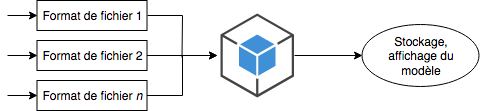
\includegraphics[width=\linewidth]{Figures/file-importation-process-native.png}
    \caption{Cas 1 : support natif des principaux formats}
    \label{fig:file-importation-process-native}
\end{figure}

Une variante est de définir un ou quelques formats principaux, complètement supportés par le logiciel. Si l'utilisateur souhaite importer un modèle stocké sous un format non pris en charge, il devra le convertir manuellement, par exemple à l'aide des fonctions d'exportation du logiciel utilisé pour sa conception.

\begin{figure}
    \centering
    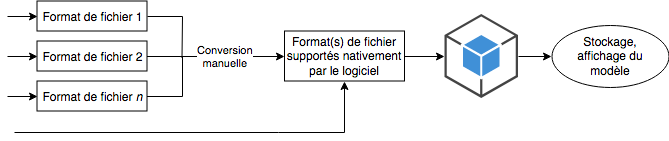
\includegraphics[width=\linewidth]{Figures/file-importation-process-manual-conversion.png}
    \caption{Cas 2 : conversion manuelle vers le(s) format(s) supportés}
    \label{fig:file-importation-process-manual-conversion}
\end{figure}

\begin{figure}
    \centering
    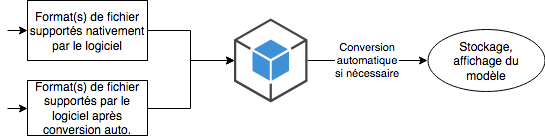
\includegraphics[width=\linewidth]{Figures/file-importation-process-auto-conversion.png}
    \caption{Cas 3 : conversion effectuée par le logiciel, si nécessaire}
    \label{fig:file-importation-process-auto-conversion}
\end{figure}


soit nativement (le logiciel sait lire différents formats), soit en se basant sur un format courant, vers lequel il est relativement aisé de convertir les autres types de fichiers au préalable.
